\documentclass[11pt]{article}

\usepackage{blindtext}
\usepackage{booktabs}
\usepackage{fullpage}
\usepackage{rotating}   
\usepackage{amsmath}
\usepackage{amssymb}
\usepackage{amsthm}
\usepackage{fancyhdr}
\usepackage{algorithm}
\usepackage{bm}
\usepackage{listings}
\usepackage{graphicx}
\usepackage{caption2}
\usepackage{subfigure}
\usepackage{float}
\usepackage{extpfeil}
\usepackage{color}
\usepackage{indentfirst} 
\usepackage[stable]{footmisc}
\usepackage[usenames,dvipsnames]{xcolor}
\usepackage[noend]{algpseudocode}

\newtheorem{theorem}{Theorem}[section]
\newtheorem{lemma}[theorem]{Lemma}
\newtheorem{corollary}[theorem]{Corollary}
\newtheorem{proposition}[theorem]{Proposition}
\newtheorem{definition}[theorem]{Definition}
\newtheorem{conjecture}[theorem]{Conjecture}
\newtheorem{remark}[subsection]{Remark}

%%
\newcommand\numberthis{\addtocounter{equation}{1}\tag{\theequation}}

%% define new symbols
\def\bx{\bm{x}}
\def\bb{\bm{b}}
\def\ba{\bm{a}}
\def\bc{\bm{c}}
\def\bf{\bm{f}}
\def\by{\bm{y}}
\def\bu{\bm{u}}
\def\bv{\bm{v}}
\def\BW{\bm{W}}
\def\BA{\bm{A}}
\def\bz{\bm{z}}
\def\BZ{\bm{Z}}
\def\BH{\bm{H}}
\def\BL{\bm{L}}
\def\BU{\bm{U}}
\def\BV{\bm{V}}
\def\BB{\bm{B}}
\def\BC{\bm{C}}
\def\BD{\bm{D}}
\def\BE{\bm{E}}
\def\BW{\bm{W}}
\def\BQ{\bm{Q}}
\def\BG{\bm{G}}
\def\BA{\bm{A}}
\def\BX{\bm{X}}
\def\BY{\bm{Y}}
\def\BQ{\bm{Q}}
\def\BI{\bm{I}}
\def\BR{\bm{R}}

%% define new brackets
\def\la{\left\langle}
\def\ra{\right\rangle}
\def\ln{\left\|}
\def\rn{\right\|}
\def\lb{\left(}
\def\rb{\right)}
\def\lsb{\left[}
\def\rsb{\right]}
\def\lcb{\left\{}
\def\rcb{\right\}}

%%
\DeclareMathOperator*{\argmin}{arg\,min}
\DeclareMathOperator*{\argmax}{arg\,max}
\setlength{\parindent}{1em}
%%
\title{Community Detection, Link Prediction and Node Classification on Ego-Facebook and Citeseer Datasets}
\author{}
\author{}
\author{Chen Liguo  17307110182\\
	Shao Yanjun  19307110036\\
    Shao Yi  19307130113}


\begin{document}
\maketitle

%------------------------------------

%-------------------------------------
%=====================
\section{Introduction}
\subsection{Problem and Background}
The final project of Social Network Mining consists of four different objectives, covering topics from basic analysis on graph structure to advanced ones such as machine learning and graph neural network (GNN). To be more specific, first of all, our team is going to make use of the topological structure of the graph to display the centrality measures, triangle count and the degree distribution in Ego-Facebook dataset. Secondly, an algorithm on \textbf{community detection} will separate the whole graph into several parties where nodes and edges in a certain party displays a high tendency of similarity. And for the most challenging part of the project, that is, to \textbf{classify nodes} and \textbf{predict links} on a graph with both topological measures and individual features of all nodes and relationship, we will implement several state-of-the-art models and discuss the pros and cons for each of them by means of comparison. Understanding how and why complicated algorithms work comes as top priority, while implementing with code and visualizing the graphs in an elegant way deserves same attention.

The whole project is launched with the help of Pytorch\footnote{https://pytorch.org/} and Neo4j\footnote{https://neo4j.com/}. Some models may require a CUDA-only version while the rest exhibits extra compatibility to run on CPU.
\begin{figure}[H]
	\centering
	\parbox{0.25\linewidth}{
		
\includegraphics[width=\linewidth]{torch.jpg}
	}\quad
	\parbox{0.2\linewidth}{
		
\includegraphics[width=\linewidth]{neo4j.jpg}
	}
\end{figure}
Neo4j is a graph database management system based on Java and accessible from software written in other languages using the Cypher query language. In Neo4j, everything is stored in the form of an edge, node, or attribute. Each node and edge can have any number of attributes. The declarative graph query language offers possibility for users to conduct expressive and efficient data querying in a property graph with high concurrency.
\subsection{Datasets Overview}
The first two parts of our final project mainly used the ego-Facebook dataset\footnote{http://snap.stanford.edu/data/ego-Facebook.html} and the rest used the Citeseer dataset\footnote{http://networkrepository.com/citeseer.php}, which has been regarded as the benchmark dataset for several topics related to graph algorithms.
\begin{figure}[H]
	\centering
	\subfigure[Ego-Facebook]{
		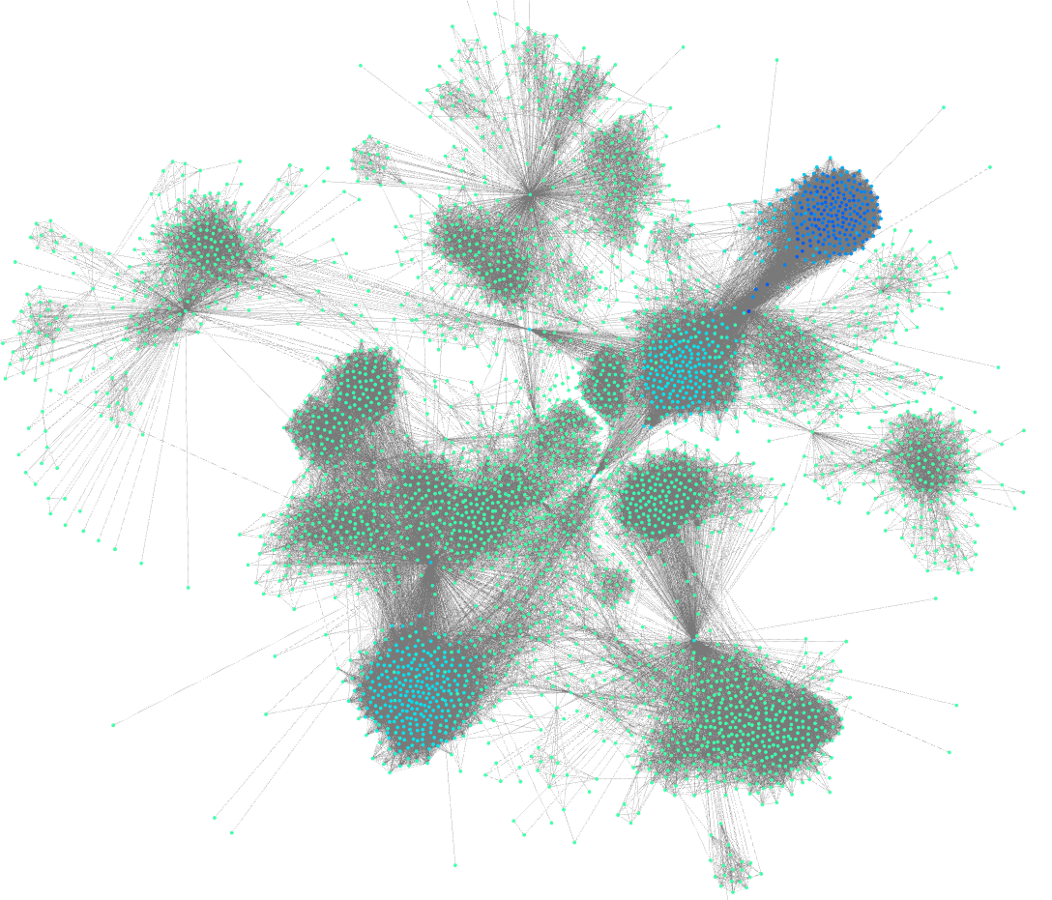
\includegraphics[width=0.3\linewidth]{graphs/overview.PNG}
	}
	\centering
	\subfigure[Citeseer]{
		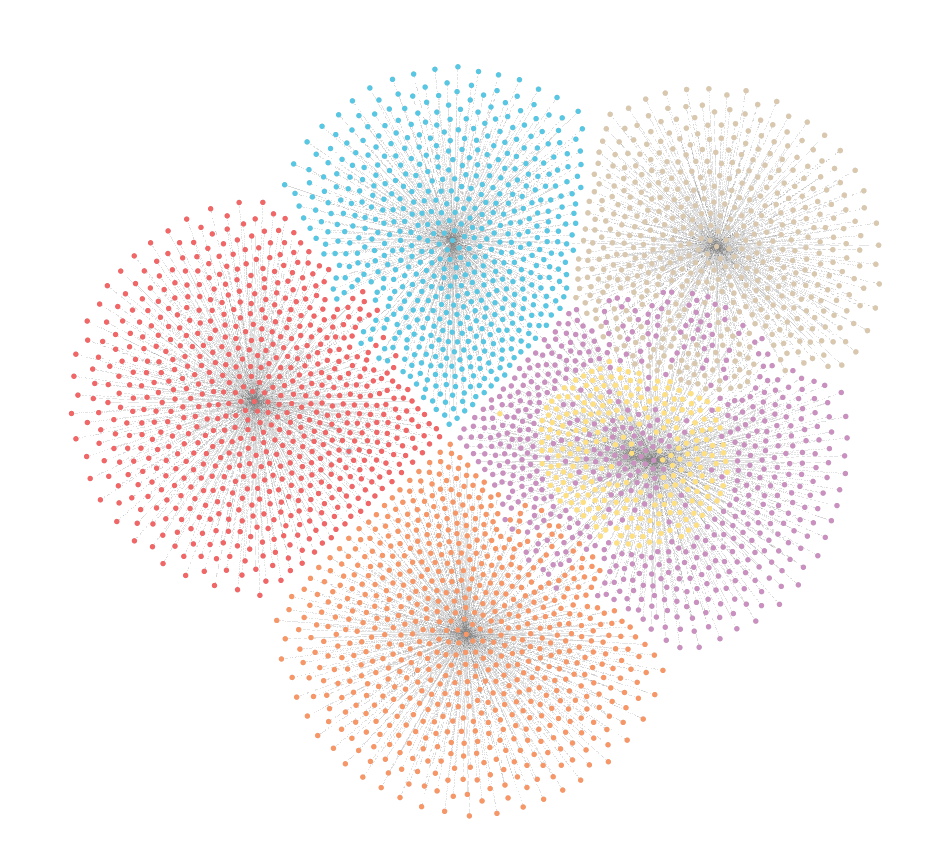
\includegraphics[width=0.25\linewidth]{citeseer/louvain.PNG}
	}
	\caption{Dataset Overview (powered by Neo4j)}
\end{figure}
The former dataset consists of 'circles' (or 'friends lists') from Facebook. It was collected from survey participants using this Facebook app. And the latter dataset consists of 3312 scientific publications classified into one of six classes. It includes publications described by a 0/1-valued word vector indicating the absence/presence of the corresponding word from the dictionary, which consists of 3703 unique words. The citation network consists of 4732 links. Here are the basic statistics and visualizations over the two datasets.
\begin{figure}[H]
	\centering
	\parbox{.4\linewidth}{
		\centering
		\begin{tabular} {cc}
			\hline\multicolumn{2}{c}{Ego-Facebook}\\
			\hline Nodes & 4039\\
			Edges & 88234\\
			Number of triangles & 1612010 \\
			Fraction of closed triangles & 0.2647\\
			Diameter (longest shortest path) & 8\\
			Average cost & 3.6925\\
		\end{tabular}
	}
\qquad\qquad
	\parbox{.4\linewidth}{
	\centering
	\begin{tabular} {cc}
		\hline\multicolumn{2}{c}{Citeseer}\\
		\hline Nodes & 3312\\
		Edges & 4732\\
		Number of triangles & 0 \\
		Fraction of closed triangles & 0\\
		Diameter (longest shortest path) & 6\\
		Average cost & 3.6541\\
	\end{tabular}
}
\caption{Network Data Statistics}
\end{figure}
\section{Degree, Centrality and Graph Analytics}
In this section, we will generally use ego-Facebook dataset for analytics.
\subsection{Zipf's Law}
Zipf's law is an empirical law that for many types of data studied in the physical and social sciences, the rank-frequency distribution exhibits an inverse relation, which belongs to a family of related discrete power law probability distributions. In most network data, the degree of each node also follows a certain power law, that is, $f(x)=ax^{-k}$. This is also true if we apply this natural rule to ego-Facebook network, because the following log-log has shown the property.
\begin{figure}[H]
	\centering
	\parbox{.45\linewidth}{
		\centering
		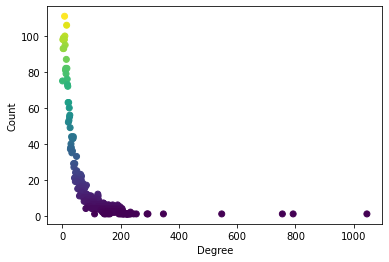
\includegraphics[width=.5\linewidth]{graphs/zipf's law1.PNG}
		\caption{Zipf's Law}
	}
	\parbox{.45\linewidth}{
	\centering
	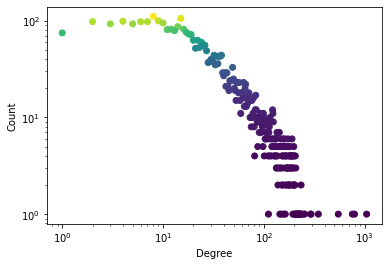
\includegraphics[width=.5\linewidth]{graphs/zipf's law.PNG}
	\caption{Zipf's Law (Under log-log)}
}
	\centering
\end{figure}
\subsection{Centrality Measures}
In graph theory and network analysis, indicators of centrality assign numbers or rankings to nodes within a graph corresponding to their network position. There are several different types of measures on node centrality described in the textbook\footnote{Zafarani, R. (2014). Social Media Mining: An Introduction (1st ed.). Cambridge University Press.} listed as follows,
\begin{figure}[H]
	\centering
	\parbox{.45\linewidth}{
		\centering
	\begin{tabular}{cc}
		\hline\multicolumn{2}{c}{Centrality}\\\hline
		Eigenvector & $c_v=\dfrac{1}{\lambda}\sum_{u\in N}c_u$\\
		PageRank & $C_p(v)=\alpha\sum_{j=1}A_{j,i}\dfrac{C_p(v_j)}{d_j^{out}}+\beta$\\
		Betweenness & $c_v=\sum_{s\ne v\ne t}\dfrac{\sigma_{s,t}(v)}{\sigma_{s,t}}$\\
		Closeness & $c_v=\dfrac{n-1}{\sum_{i\ne j}l_{i,j}}$	
	\end{tabular}
\caption{Table}
}
	\parbox{.45\linewidth}{
		\centering
	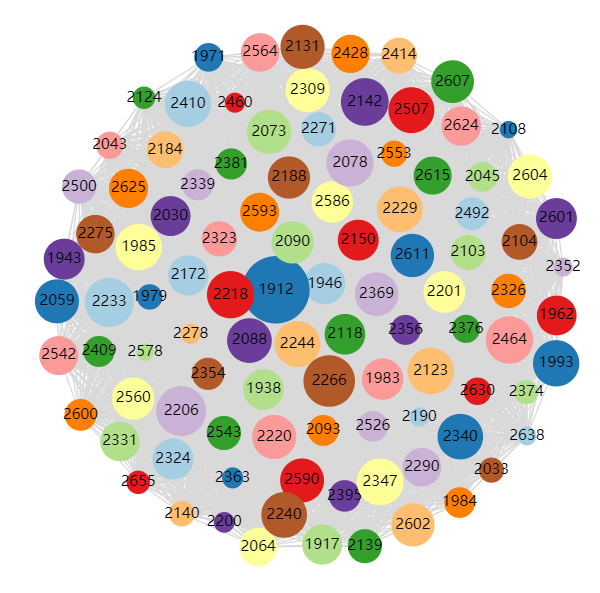
\includegraphics[width=0.5\linewidth]{graphs/eigenvector centrality.PNG}
\caption{Eigenvector Centrality}	
}
\end{figure}
We will only list top 5 nodes with respect to each centrality properties in order to get a clear overview of the difference between measures.
\begin{table}[H]
	\centering
	\parbox{.2\linewidth}{
		\centering
	\begin{tabular}{cc}
		\hline ID & Eigenvector\\\hline
		1912 & 296.5844\\
		2266 & 254.0166\\
		2206 & 250.4103\\
		2233 & 248.8579\\
		2142 & 245.7742
	\end{tabular}
}\quad
	\parbox{.2\linewidth}{
	\centering
	\begin{tabular}{cc}
		\hline ID & PageRank\\\hline
		3437 & 29.680\\
		107 & 27.084\\
		1684 & 24.785\\
		0 & 24.498\\
		1912 & 15.061
	\end{tabular}
}\quad
	\parbox{.2\linewidth}{
	\centering
	\begin{tabular}{cc}
		\hline ID & Betweenness\\\hline
		107 & 3916560\\
		1684 & 2753587\\
		3437 & 1924506\\
		1912 & 1868918\\
		1085 & 1214578
	\end{tabular}
}\quad
	\parbox{.2\linewidth}{
	\centering
	\begin{tabular}{cc}
		\hline ID & Closeness\\\hline
		107 & 0.4597\\
		58 & 0.3974\\
		428 & 0.3948\\
		563 & 0.3939\\
		1684 & 0.3936
	\end{tabular}
}
\caption{Difference}
\end{table}
As we can see from Table 1, Eigenvector Centrality cannot capture the essense of the topological structure of the network because all the nodes with high Eigenvector rankings gather in small clique. With iteration going on, all the centrality weights stream into several closely-related neighbour nodes, making them outrageously too powerful.
%-------------------------------------
%=====================
\end{document}
